%!TEX root = paper.tex

\section{Markov-Chain Monte Carlo}\label{sec:mcmc}

To evaluate the quality of the covariance estimates produced by our method, we used Markov-Chain Monte Carlo (MCMC) as a benchmark for the ``true'' distribution of the logistic regression weights $(w_0, w_1, w_2)$.  \texttt{R}

\begin{figure}
\centering
	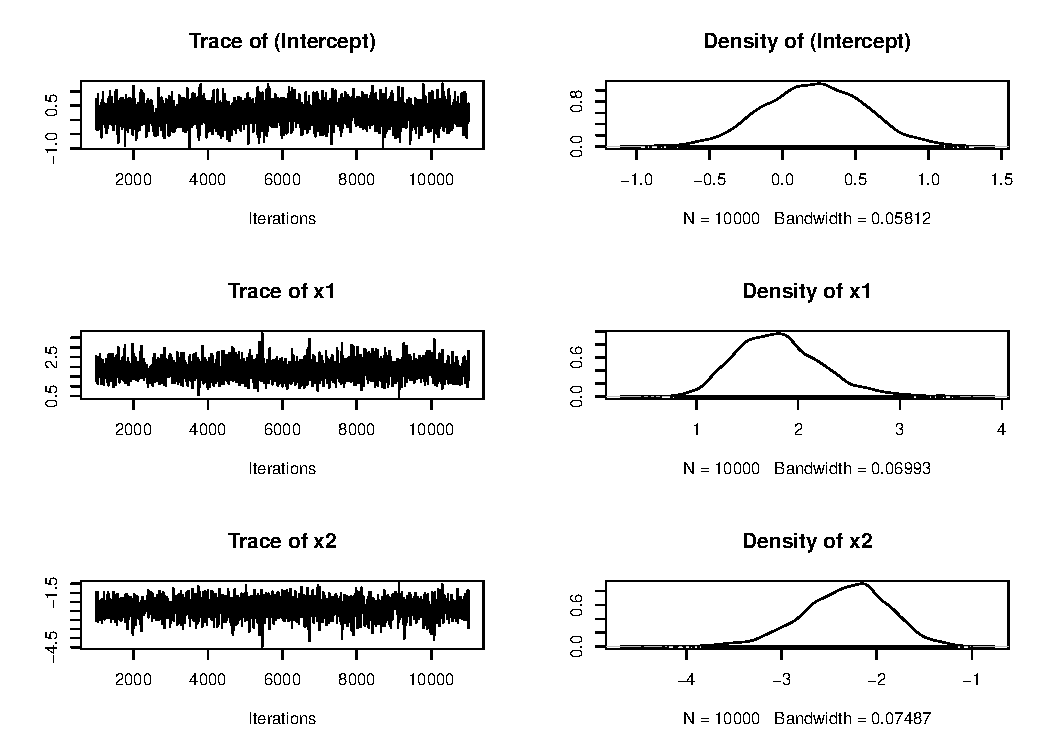
\includegraphics[height=120mm]{figures/mcmc_uniform.pdf}
    \caption{MCMC simulations of logistic regression weights for dataset 1, and corresponding marginal density plots, assuming 
    an improper uniform prior. 10,000 iterations total.}  \label{fig:mcmc_iterations}  
\end{figure}

\begin{figure}
\centering
	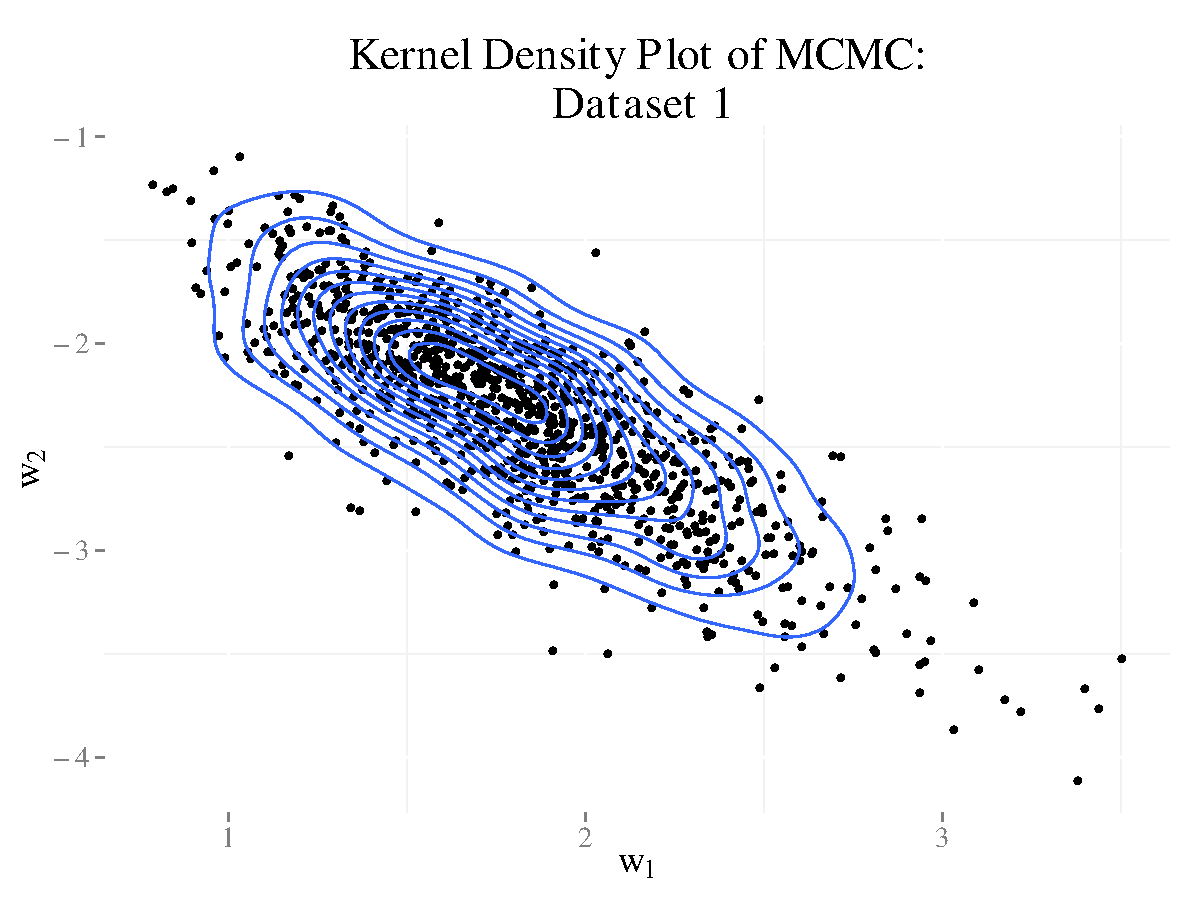
\includegraphics[height=120mm]{figures/mcmc_uniform_2d.pdf}
    \caption{MCMC simulations of logistic regression weights for dataset 1, and corresponding kernel density plot, assuming 
    an improper uniform prior.  Subset of 1,000 out of 10,000 total iterations shown.}  \label{fig:mcmc_kernel}  
\end{figure}

\begin{figure}
\centering
	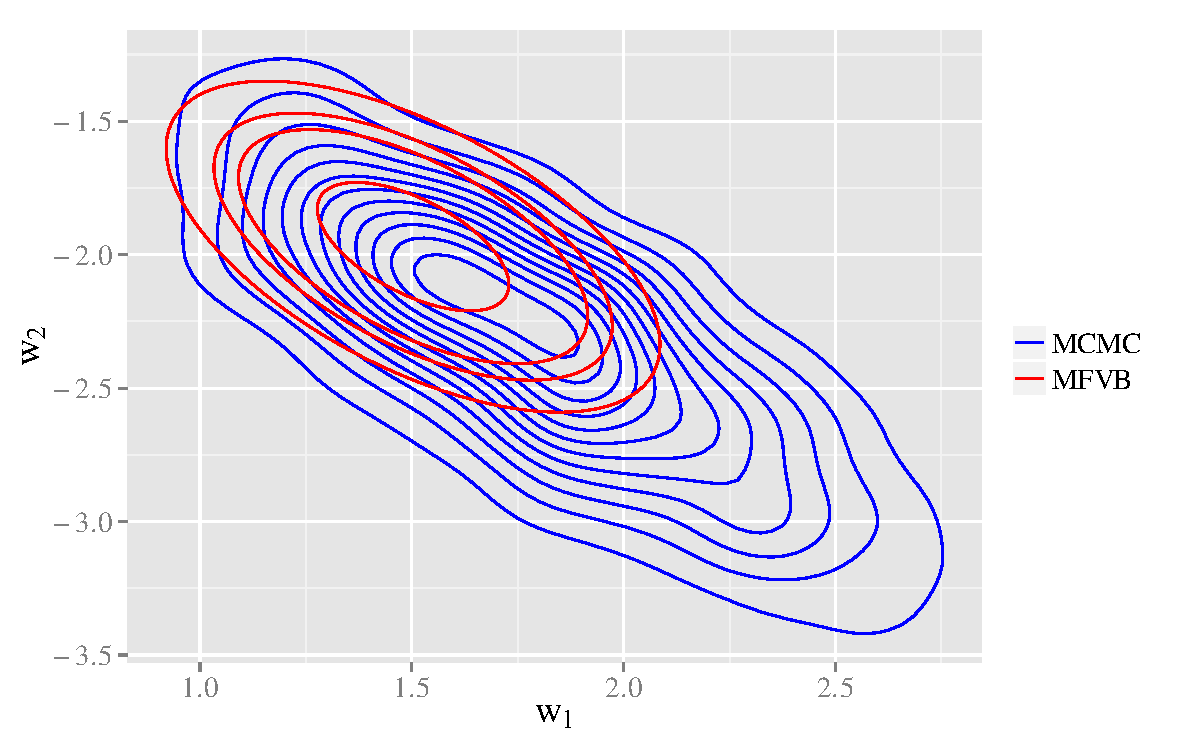
\includegraphics[height=120mm]{figures/mcmc_uniform_mfvb.pdf}
    \caption{Comparison of logistic regression point estimate, kernel density plot of MCMC simulations, and posterior density of
    MFVB logistic regression (vectorized function), for dataset 1.   Contours of MFVB logistic regression indicate
    50\%, 90\%, 95\%, and 99\% confidence intervals for the bivariate normal $\mathcal{N}(\M{w}_{N},\M{V}_N)$.
    Mean values for MCMC and MFVB are also included.}  \label{fig:mcmc_mfvb}  
\end{figure}